\chapter{Conclusion and future work}


Nowadays, decision-making processes are changing significantly. A wide range of tools is designed and created every day to help with this complex task. The project ITRC-Mistral aims to help policymakers, governments, businesses and stakeholders of the telecommunications sector to assess the performance and impact of long-term plans. This Master’s Thesis contributes to the model MINERVA to implement and test different coverage obligation sets for the 700 MHz band in the UK. \par

Firstly, the contributions to the project revolve around three main issues: the new capacity expansion strategy (\textit{\guillemotleft 700 MHz densification\guillemotright }), the coverage obligation sets inspired in the real obligations imposed with the allocation of 800 MHz spectrum (\guillemotleft \textit{Priority areas first\guillemotright , \guillemotleft Less profitable areas first\guillemotright , \guillemotleft Only rural areas\guillemotright  and \guillemotleft Nation-balanced\guillemotright }), and the new visualization module, which creates data files, diagrams, histograms, coloured maps and gifs automatically after the simulation.\par

Secondly, the implemented functions were tested to analyse how the coverage obligations influence the pace of the rollouts. An analysis of how the infrastructure is deployed when the telecom operator only has the 700 MHz band was carried out. Additionally, a comparison was performed with other capacity-expansion strategies, such as small cells, traditional telecommunication spectrum or a combination of both. This comparison allows assessing the impact that this radio frequency band may have on the deployment of future 5G networks.\par

Finally, the implications that coverage obligations have on the evolution of the capacity deployed and end-user speeds were tested. The results suggest that the sequence in which a telecom operator is compelled to invest can have a great impact on both the end-user speed and costs and on the differences across regions.\par




\subsubsection*{1. On the impact of new spectrum for the future rollout of 5G.}
\addcontentsline{toc}{subsubsection}{1. On the impact of new spectrum for the future rollout of 5G.}
According to the forecasted traffic growth, the demand that we expect in coming years is much higher than the capacity that current base stations can provide. To face this challenge, a telecom operator can either seek more spectrum in the following auctions or build more base stations, so that it can boost the capacity by increasing the density of the assets (and therefore reducing the number of users per base station).\par

Implications of both solutions are tested using several capacity-expansion strategies. \textit{\guillemotleft Spectrum integration\guillemotright } and \textit{\guillemotleft 700 MHz spectrum integration\guillemotright } strategies cannot build new assets, but only add new spectrum bands to the existing ones. The \textit{\guillemotleft small cells strategy\guillemotright } allow to create new assets, but only using small cells. Finally, the \textit{\guillemotleft hybrid strategy\guillemotright } allows to create new assets as well as to upgrade existing ones, using all the spectrum bands allocated for telecommunication services. This work identified that no strategy considered the possibility of only creating assets of the 700 MHz band and, thus, the \textit{\guillemotleft 700 MHz densification\guillemotright } strategy was defined. \par

There is a technological limit to the network capacity expansion strategies that rely exclusively on 700 MHz. The results show that this band could not provide enough capacity in all the areas and should be deployed in combination to the bigger bandwidths of the 5G: The 50 MHz blocks of the 3.5 GHz and the 25 MHz blocks in the 3.7 GHz small cells. A strategy that combines these high bandwidths, especially the 3.5GHz band, and the \textit{\guillemotleft 700 MHz densification\guillemotright }, would reduce costs and have enough capacity to cover even the more dense populations. \par

In other words, according to the model used in this Thesis, it is not possible to satisfy the overall demand of capacity in ten years by just upgrading existing assets. Therefore, it becomes necessary to build any kind of new base station to densify the network, either using macrocells or small cells. Thus, there are two important conclusions for policy-makers. First, facilitation the creation of new base stations is highly relevant since this is a precondition to giving enough end-user speed to the whole country. Second, allocating frequency bands (such as 3.5 GHz) with larger bandwidth is equally important because they provide a wider capacity with the same site density than the traditional telecommunication bands.\par








\subsubsection*{2. On the impact of the coverage obligation options.}
\addcontentsline{toc}{subsubsection}{2. On the impact of the coverage obligation options.}
The second part of the work is focused on analysing the impact of the coverage obligation sets. A coverage obligation is a combination of settings that describe the commitments that a policy-maker could compel telecom operators to achieve.\par

This Thesis has developed and implemented five coverage obligation options, but the code allows to configure more. Four out of the five coverage obligations were inspired in the real commitments for 800MHz in Spain, the UK, France and Germany, and the fifth was already preconfigured in the original NISMOD project. \par

It is important to see the impact that coverage obligations have in the network capacity and, therefore, in the end-user speed. Telecom assets require a high investment. Consequently, telecom operators prefer to invest first in urban geotypes since they are the most profitable and leave rural geotypes least. This work considers that a telecom operator would start to invest in most populated regions and would sort them in descending order. For this reason, typically, the curve that represents the end-user speed as of the population density is as follows:\par


%%%%%%%%%%%%%%%%%%%% Figure/Image No: 1 starts here %%%%%%%%%%%%%%%%%%%%

\begin{figure}[H]
	\begin{Center}
		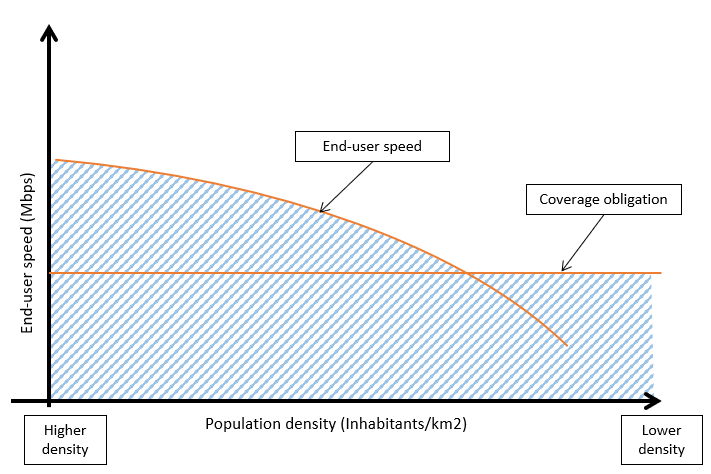
\includegraphics[width=4.29in,height=2.86in]{./media/image103.png}
		\caption{Impact of the coverage obligations in the end-user speed. Source: Author}
	\end{Center}
\end{figure}


%%%%%%%%%%%%%%%%%%%% Figure/Image No: 1 Ends here %%%%%%%%%%%%%%%%%%%%



In respect of the specific coverage obligation sets of the Thesis, the results show that they have a strong impact on the development of the regions. Coverage obligations can be divided into three groups according to the order of investment. The difference between them is that some of them (\textit{\guillemotleft Priority areas first\guillemotright } and\textit{ \guillemotleft Less profitable areas first\guillemotright }) oblige a minimum speed for a minimum percentage of the population and a specific order of deployment, while others (\textit{\guillemotleft More profitable first\guillemotright } and \textit{\guillemotleft Nation-balanced\guillemotright }) only enforce a minimum speed for a minimum percentage of the population.\textit{ \guillemotleft Only rural areas\guillemotright } just include a small proportion of the population.\par

Conclusions in this chapter depend mainly on the capacity expansion strategy selected. For those strategies that are capped technically because they do not have enough radio frequency bands to use, or because they cannot build new assets in places that have no base stations, the order of investment is not the key for the development of the country’s network. As they can invest sooner or later in all the regions, because the budget is not their basic restriction, the capacity margin and the percentage of population covered in each region is pretty similar in all of them.\par

The differences between coverage obligation alternative become important while focusing on the evolution over the years. For instance, analysing the graphs of the \textit{\guillemotleft 700 MHz densification\guillemotright } strategy simulations, the differentiation of both types of coverage obligations becomes very clear. The final result is the same, but while the first group uses a third of the total investment (£1billion, which is the budget for 2 years) to invest in regions that have 10$\%$  of the population, the other strategies have already invested in regions that sum 60$\%$  of the population.\par

On the contrary, capacity expansion strategies that can cover 100$\%$  of the population are more affected by the coverage obligation order, since they could carry out significant investments in the less profitable regions. In fact, results of the simulations using the \guillemotleft Hybrid strategy\guillemotright  are completely different depending on the coverage obligation chosen. Strategies that force the operator to firstly invest a high amount in less-profitable areas are heavily penalized compared to strategies that allow the telecom operator to choose. For instance, the first group of obligations need all the budget to just raise the percentage until the 45$\%$  of the population, while the other group raises the percentage until 90$\%$ , just using the same budget. \par

\textit{A priori}, it seems more interesting to let the telecom operator decide in which regions it is better for it to start investing, provided they meet the obligations before the end of the period. In this case, obligations such as \textit{\guillemotleft More profitable first\guillemotright } and \textit{\guillemotleft Nation-balanced\guillemotright } would have better results. However, deploying a new telecommunications infrastructure is expensive and deadlines for coverage obligations are scheduled for several years. If there is no forced order and there are no intermediate milestones, policy-makers have no mechanism to compel the telecom operator to increment the investment rate.\par

On the other hand, coverage obligations such as \textit{\guillemotleft Priority areas first\guillemotright ,} \textit{\guillemotleft Only rural areas\guillemotright  }and\textit{ \guillemotleft Less profitable areas first\guillemotright } oblige the telecom operator to reach a minimum percentage of population covered in a group of regions (normally the least profitable ones) before investing in the most profitable ones.\par

These strategies of the policy-maker penalise the development of the telecommunications network but have two significant advantages. First, the telecom operator is interested in deploying new assets as soon as possible, because the faster it invests in the less profitable areas, the quicker it starts investing in the more profitable ones. Second, these coverage obligations have intermediate milestones and, therefore, policy-makers do not have to wait until the end of the period to evaluate if they have to sanction the telecom operator.\par

As a final conclusion, policy-makers are responsible for choosing an option in order to fulfil coverage obligations. Additionally, it is important to note that this decision will have a great impact on the development of the telecommunication services infrastructure. In as much as coverage obligations are related to the price of the spectrum, depending on how aggressive they are, prices may be affected. \par

This approach would require considering three types of scenarios, which would depend on the extent on coverage obligations. Firstly, a fundraising scenario, in which there will not be any coverage obligations. Therefore, telecom operator would pay higher bids to receive spectrum. Secondly, a long-term scenario, where telecom operators would have to comply with a minimum end-user speed in a future date. In this scenario, telecom operators would need a smaller investment. Finally, a short-term scenario, in which the investment would be even smaller, to the extent that they would have to invest in prioritizing the less-profitable regions of the country.\par



%%%%%%%%%%%%%%%%%%%% Table No: 2 starts here %%%%%%%%%%%%%%%%%%%%


\begin{table}[H]
 			\centering
\begin{tabular}{p{1.05in}p{1.20in}p{1.15in}p{1.42in}}
\hline
%row no:1
\multicolumn{1}{|p{1.05in}}{\Centering \textbf{Scenario}} & 
\multicolumn{1}{|p{1.20in}}{\Centering \textbf{Expected bids}} & 
\multicolumn{1}{|p{1.15in}}{\Centering \textbf{Forced order}} & 
\multicolumn{1}{|p{1.42in}|}{\Centering \textbf{Equalising factor}} \\
\hhline{----}
%row no:2
\multicolumn{1}{|p{1.05in}}{\Centering Fundraising} & 
\multicolumn{1}{|p{1.20in}}{\Centering High} & 
\multicolumn{1}{|p{1.15in}}{\Centering No} & 
\multicolumn{1}{|p{1.42in}|}{\Centering Low} \\
\hhline{----}
%row no:3
\multicolumn{1}{|p{1.05in}}{\Centering Long-term} & 
\multicolumn{1}{|p{1.20in}}{\Centering Medium} & 
\multicolumn{1}{|p{1.15in}}{\Centering No} & 
\multicolumn{1}{|p{1.42in}|}{\Centering High} \\
\hhline{----}
%row no:4
\multicolumn{1}{|p{1.05in}}{\Centering Short-term} & 
\multicolumn{1}{|p{1.20in}}{\Centering Low} & 
\multicolumn{1}{|p{1.15in}}{\Centering Yes} & 
\multicolumn{1}{|p{1.42in}|}{\Centering High} \\
\hhline{----}

\end{tabular}
 \end{table}


%%%%%%%%%%%%%%%%%%%% Table No: 2 ends here %%%%%%%%%%%%%%%%%%%%











\vspace{\baselineskip}
\subsection*{Future work}
\addcontentsline{toc}{subsection}{Future work}
During the development of this Master’s Thesis, some lines for future work and some possible improvements applicable to the code have been identified.\par

First. MINERVA generalizes the profitability of the investment in each region and assumes that the more densely populated a region is, the more profitable are the investments. Nevertheless, the capacity obtained from the propagation model depends on the geotype and this assumption is not always true. This matter requires a detailed study so that the model can really estimate in which order would the telecom operator make the investments.\par

Second. This project uses three types of geotypes, sorted by their population density, and each geotype has been modelled with different propagation characteristics. The way that the capacity curves are calculated causes that, within each geotype, most densely populated areas have larger capacity deficits. Regions in the border have similar demand since they have a similar population density, but the most densely populated areas of each geotype have considerably lower capacity expectations because people are expected to be less concentrated than in bigger urban centres. A possible solution could be to define more geotypes, so differences between them become lower. \par

Third. For each year of the simulation, MINERVA compares the capacity of the assets of each region against the minimum end-user speed of the coverage obligation. Once all the regions are satisfied, it starts checking if the capacity is enough to satisfy the real demand of the population. In consequence, the model makes no investments to fulfil the second speed until every region has its obligations met. There are two more realistic approaches for this mechanism:\par

\begin{itemize}
	\item Set a minimum percentage of the budget that is only available for investments made to meet the real demand. Thus, even when coverage obligations are wide and investments start in the less profitable regions, the most-profitable ones can receive some investment from the first year. \par

	\item Use the variable time and distribute the investment equally or proportionally over the years that the coverage obligation lasts.
\end{itemize}\par

The following graph represents a realistic distribution of the investments over the years:\par



%%%%%%%%%%%%%%%%%%%% Figure/Image No: 2 starts here %%%%%%%%%%%%%%%%%%%%

\begin{figure}[H]
	\begin{Center}
		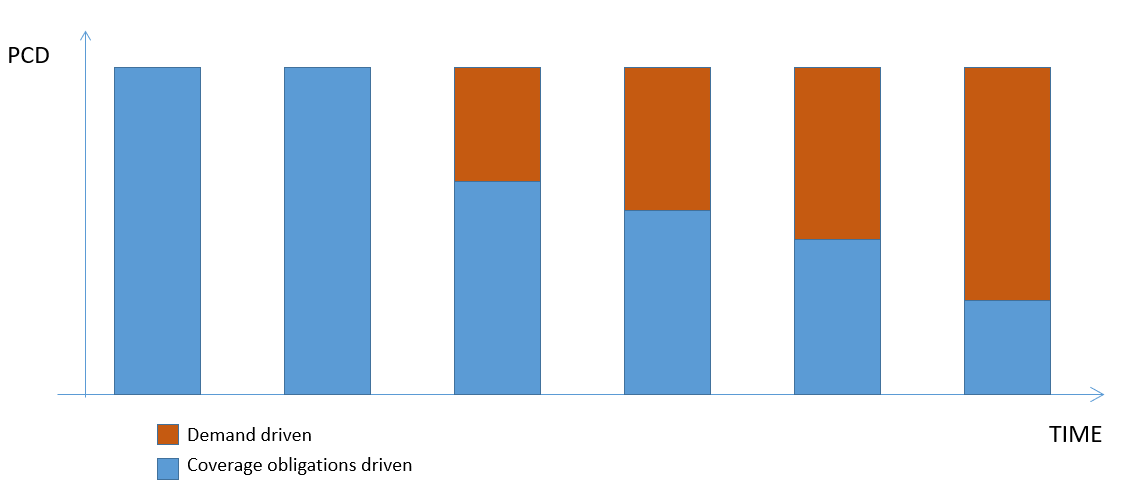
\includegraphics[width=4.6in,height=2.0in]{./media/image104.png}
		\caption{Impact of the coverage obligations in the end-user speed. Source: Author}

	\end{Center}
\end{figure}


%%%%%%%%%%%%%%%%%%%% Figure/Image No: 2 Ends here %%%%%%%%%%%%%%%%%%%%

\par

Fourth. Having information at a PCD level is not detailed enough for the propagation model. Obtaining information about the percentage of the urban, suburban and rural area of each PCD would allow MINERVA to have more precise simulations. The same issue applies to the percentage of penetration of mobile services. It is currently set at 80$\%$ , but this percentage shall depend on the geotype since they use mobile services for different use cases.\par

Fifth. This work only takes into account the traditional traffic generated by end users but does not consider the other possible use cases of the 5G networks: Massive machine-type communications and Ultra-reliable and low latency communications. Each use case conditions 5G networks in a different way and all of them should be considered in the model. Thus, MINERVA should consider issues such as that some traffic types will demand low rate connections and that IoT communications could exceed the maximum simultaneous connections allowed to a base station. MINERVA should include models of these types of traffic and consider them in the decision module.\par


\vspace{\baselineskip}











%%\vspace{\baselineskip}\section*{Conclusion}
%%\addcontentsline{toc}{section}{Conclusion}
%Nowadays, the decision-making process is changing significantly in every sector of the industry. A wide range of tools is designed and created every day to help with this key and risky task. The MINERVA project helps policymakers, governments, businesses and stakeholders of the telecommunications sector to assess the performance and impact of long-term plans. This Master’s Thesis is focused on two main topics: Contributing to the MINERVA project and benefit from the resources provided by the project, in order to draw worthwhile conclusions regarding it.\par
%
%First, three new features were included: the new capacity expansion strategy (\textit{\guillemotleft 700 MHz densification\guillemotright }), the coverage obligation options inspired in real obligations regarding the first digital dividend (\guillemotleft \textit{Priority areas first\guillemotright , \guillemotleft Less profitable areas first\guillemotright , \guillemotleft Only rural areas\guillemotright  and \guillemotleft Nation-balanced\guillemotright }), and the new visualization module, which creates data files, diagrams, histograms, coloured maps and gifs automatically after the simulation.\par
%
%Second, these features were applied to analyse its impact on the deployment speed.\ Hence, an analysis of how the infrastructure develops when the telecom operator only has the 700 MHz band was carried out.  Additionally, a comparison was performed with other band combination scenarios, such as using small cells, traditional telecommunication spectrum or a union of both, in order to understand which is the impact that this radio frequency band can have in the deployment of the 5G networks.\par
%
%Afterwards, the implications that coverage obligations have on the evolution of the capacity deployed and end-user speeds were tested. As we have already seen, the sequence in which a telecom operator is compelled to invest can make a great impact on reducing or increasing the end-user speed differences between regions.\par
%
%
%
%
%\subsubsection*{1. On the impact of deploying 5G at 700 MHzthe capacity expansion strategies.}
%\addcontentsline{toc}{subsubsection}{1. On the impact of the capacity expansion strategies.}
%A capacity expansion strategy is a set of radio frequency bands that the telecom operator could use combined with the preferred order in which it would like to start building new assets when there is a lack of capacity.\par
%
%During the development of the thesis, it was noted that the demand that we expect in some years is much higher than the capacity that current base stations can provide. Therefore, there are only two possible solutions for a telecom operator: Biding for more spectrum in the following auctions, so that it can increase the capacity using more bandwidth, or building more base stations, so that it can boost the capacity by increasing the density of the assets and reducing the number of users per base station.\par
%
%The capacity expansion strategies tested in this thesis have been selected to analyse the implications of both solutions. \guillemotleft Spectrum integration\guillemotright  and \guillemotleft 700 MHz spectrum integration\guillemotright  cannot build new assets, they can just add new spectrum bands to the existing ones. \guillemotleft 700 MHz densification\guillemotright  and \guillemotleft Small cells strategy\guillemotright  allow to create new assets, but they can only use the 700 MHz band and small cells technology, respectively. Finally, \guillemotleft Hybrid strategy\guillemotright  is a strategy which allows to create new assets as well as to upgrade existing ones, using all the spectrum bands allocated for telecommunication services.\par
%
%This thesis uses a predefined propagation model that estimates the capacity of the network depending on the site density, the geotype of the PCD and the bandwidth available. Capacity calculations with 700 MHz, 800 MHz and 2.6 GHz bands use a bandwidth of 2x10 MHz, which has capacity limitations compared to higher frequency bands. The 3.5 GHz band has a considerable available bandwidth, so estimations use blocks of 50 MHz and small cells use the 3.7 GHz band with blocks of 25 MHz. These high bandwidths make the capacity of these bands especially interesting for areas with a high demand for end-user speed, such as areas with a high population density.\par
%
%The\ first output of the simulations is that just using the 700, 800 and 2600 MHz bands is not enough to provide sufficient user-speed rates in some areas.  three types of geotypes have been used, sorted by their population density, and each geotype has been modelled with different propagation characteristics. This causes that the regions that are next to the limit to the upper geotype could experience some capacity limitations. The reason is that these regions have similar demand since they have a similar population density, but they have considerably lower capacity expectations because people are expected to be less concentrated than in great urban centres (Their geotype estimates less capacity).\par
%
%The impact of only enable the usage of the 700 MHz band would imply in the telecom operator was also tested. Outcomes show that this band could not provide enough capacity in some regions form all kinds of geotypes. After analysing the results, an unexpected conclusion was reached. In fact, regions from suburban and rural geotypes are more penalised than regions from the urban geotype, due to the propagation model.\par
%
%To sum up, the results show that, using the model of the thesis, it is not possible to satisfy the overall demand of capacity in ten years by just upgrading existing assets and that it is necessary to build any kind of new base station either using macrocells or small cells. Thus, there are two important issues that the telecom operator has to consider. First, it has to be permitted to create new base stations since this is the first requirement to give enough end-user speed to the whole country. Second, it should use at least one of the bands that have the larger bandwidth (macrocells with 3.5GHz or small cells with 3.7GHz) because they provide a wider capacity with the same site density than the traditional telecommunication bands.\par
%
%
%
%
%\subsubsection*{2. On the impact of the coverage obligation options.}
%\addcontentsline{toc}{subsubsection}{2. On the impact of the coverage obligation options.}
%The second part of the work is focused on analysing the impact of the coverage obligation options. A coverage obligation option is a combination of settings that describe the commitments that a policymaker could compel telecom operators to achieve.\par
%
%This thesis has five coverage obligation options predefined, but more can be configured. Four out of five of these obligations were inspired in the engagements of the 800MHz in Spain, the UK, France and Germany and the fifth was already preconfigured in the original NISMOD project. Policy-makers developed these coverage obligations aiming to reduce the end-user speed differences between regions of the same country. This paper focuses on testing how effective these obligations are and the advantages and disadvantages of each of these measures.\par
%
%Before beginning with the analysis of each coverage obligation, it is important to see the impact that coverage obligations have in the network capacity and, therefore, in the end-user speed. Telecom assets require a high investment. Consequently, telecom operators prefer to invest in those places that are profitable for them. According to the analysis of chapter 3, urban geotypes are the most profitable ones, while rural geotypes are the least. This paper considers that a telecom operator would start investing in regions with more population density and would sort them in descending order. For this reason, typically, the curve that represents the end-user speed of the inhabitants of a country depending on the population density of the area where they live can be represented using the following graph:\par
%
%
%
%%%%%%%%%%%%%%%%%%%%% Figure/Image No: 6 starts here %%%%%%%%%%%%%%%%%%%%
%
%\begin{figure}[H]
	%\begin{Center}
		%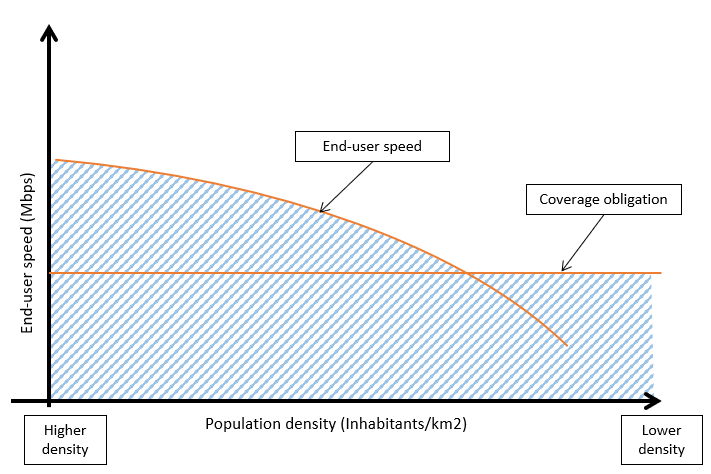
\includegraphics[width=4.29in,height=2.86in]{./media/image103.png}
		%\caption{Impact of the coverage obligations in the end-user speed. Source: Author}
	%\end{Center}
%\end{figure}
%
%
%%%%%%%%%%%%%%%%%%%%% Figure/Image No: 6 Ends here %%%%%%%%%%%%%%%%%%%%
%
%Generally, most of the inhabitants of the densely populated regions have higher end-user speeds than the minimum speed required by the coverage obligation and, therefore, coverage obligations have no benefits for them. By contrast, the regions that have less population and become more rural, have less access to the latest radio networks technology and, hence, have a worse internet connection. Coverage obligations decrease the internet access quality gap and homogenize the benefits of the telecommunications infrastructure along the country.\par
%
%In respect of the specific coverage obligation options of the thesis, results show that they have a strong impact on the development of the regions. Coverage obligations can be divided into three groups according to the order of investment. Firstly, those that bind a different order of investment than the suitable for the operator (\textit{\guillemotleft Priority areas first\guillemotright } and\textit{ \guillemotleft Less profitable areas first\guillemotright }). Secondly, those that let the operator decide (\textit{\guillemotleft More profitable first\guillemotright } and \textit{\guillemotleft Nation-balanced\guillemotright }). Thirdly, \textit{\guillemotleft Only rural areas\guillemotright }, which does not belong completely to any of the groups since it just compels to begin by the rural areas, but they just include a small proportion of the population.\par
%
%The difference between them is that coverage obligations of the first group oblige a minimum speed for a minimum percentage of the population and a specific order of deployment, while the second group only enforces a minimum speed for a minimum percentage of the population.\par
%
%Conclusions in this chapter depend mainly on the capacity expansion strategy selected. For those strategies that are capped technically because they do not have enough radio frequency bands to use, or because they cannot build new assets in places that have no base stations, the order of investment is not the key for the development of the country’s network. As they can invest sooner or later in all the regions, because the budget is not their basic restriction, the capacity margin and the percentage of population covered in each region is pretty similar in all of them.\par
%
%The differences between coverage obligation alternative become important while focusing on the evolution over the years. For instance, analysing the graphs of the \textit{\guillemotleft 700 MHz densification\guillemotright } strategy simulations, the differentiation of both types of coverage obligations explained above becomes very clear. The final result is the same, but while the first group uses a third of the total investment (£1billion, which is the budget for 2 years) to invest in regions that have 10$\%$  of the population, the other strategies have already invested in regions that sum 60$\%$  of the population.\par
%
%On the contrary, capacity expansion strategies that can cover 100$\%$  of the population are more affected by the coverage obligation order, since they could carry out significant investments in the less profitable regions. In fact, results of the simulations using the \guillemotleft Hybrid strategy\guillemotright  are completely different depending on the coverage obligation chosen. Strategies that force the operator to firstly invest a high amount in less-profitable areas are heavily penalized compared to strategies that allow the telecom operator to choose. For instance, in the graphs of the previous chapter, the first group of obligations need all the budget to just raise the percentage until the 45$\%$  of the population, while the other group raises the percentage until 90$\%$ , just using the same budget. \par
%
%\textit{A priori}, it seems more interesting to let the telecom operator decide in which regions it is better for it to start investing, provided they meet the obligations before the end of the period. In this case, obligations such as \textit{\guillemotleft More profitable first\guillemotright } and \textit{\guillemotleft Nation-balanced\guillemotright } would have better results. However, deploying a new telecommunications infrastructure is expensive and deadlines for coverage obligations are scheduled for several years. If there is no forced order and there are no intermediate milestones, policy-makers have no mechanism to compel the telecom operator to increment the investment rate.\par
%
%On the other hand, coverage obligations such as \textit{\guillemotleft Priority areas first\guillemotright ,} \textit{\guillemotleft Only rural areas\guillemotright  }and\textit{ \guillemotleft Less profitable areas first\guillemotright } oblige the telecom operator to reach a minimum percentage of population covered in a group of regions (normally the least profitable ones) before investing in the most profitable ones.\par
%
%These strategies of the policy-maker penalize the development of the telecommunications network but have two significant advantages. First, the telecom operator is interested in deploying new assets as soon as possible, because the faster it invests in the less profitable areas, the quicker it starts investing in the more profitable ones. Second, these coverage obligations have intermediate milestones and, therefore, policy-makers do not have to wait until the end of the period to evaluate if they have to sanction the telecom operator.\par
%
%As a final conclusion, the policymaker is responsible for choosing an option in order to fulfil coverage obligations. Additionally, it is important to note that this decision will have a great impact on the development of the telecommunication services infrastructure. In as much as coverage obligations are related to the price of the spectrum, depending on how aggressive they are, prices may be affected. \par
%
%This approach would require considering three types of scenarios, which would depend on the extent on coverage obligations. Firstly, a fundraising scenario, in which there will not be any coverage obligations. Therefore, telecom operator would pay higher bids to receive spectrum. Secondly, a long-term scenario, where telecom operators would have to comply with a minimum end-user speed in a future date. In this scenario, telecom operators would need a smaller investment. Finally, a short-term scenario, in which the investment would be even smaller, to the extent that they would have to invest in prioritizing the less-profitable regions of the country.\par
%
%
%
%%%%%%%%%%%%%%%%%%%%% Table No: 2 starts here %%%%%%%%%%%%%%%%%%%%
%
%
%\begin{table}[H]
 			%\centering
%\begin{tabular}{p{1.05in}p{1.20in}p{1.15in}p{1.42in}}
%\hline
%%row no:1
%\multicolumn{1}{|p{1.05in}}{\Centering \textbf{Scenario}} & 
%\multicolumn{1}{|p{1.20in}}{\Centering \textbf{Expected bids}} & 
%\multicolumn{1}{|p{1.15in}}{\Centering \textbf{Forced order}} & 
%\multicolumn{1}{|p{1.42in}|}{\Centering \textbf{Equalising factor}} \\
%\hhline{----}
%%row no:2
%\multicolumn{1}{|p{1.05in}}{\Centering Fundraising} & 
%\multicolumn{1}{|p{1.20in}}{\Centering High} & 
%\multicolumn{1}{|p{1.15in}}{\Centering No} & 
%\multicolumn{1}{|p{1.42in}|}{\Centering Low} \\
%\hhline{----}
%%row no:3
%\multicolumn{1}{|p{1.05in}}{\Centering Long-term} & 
%\multicolumn{1}{|p{1.20in}}{\Centering Medium} & 
%\multicolumn{1}{|p{1.15in}}{\Centering No} & 
%\multicolumn{1}{|p{1.42in}|}{\Centering Medium} \\
%\hhline{----}
%%row no:4
%\multicolumn{1}{|p{1.05in}}{\Centering Short-term} & 
%\multicolumn{1}{|p{1.20in}}{\Centering Low} & 
%\multicolumn{1}{|p{1.15in}}{\Centering Yes} & 
%\multicolumn{1}{|p{1.42in}|}{\Centering High} \\
%\hhline{----}
%
%\end{tabular}
 %\end{table}
%
%
%%%%%%%%%%%%%%%%%%%%% Table No: 2 ends here %%%%%%%%%%%%%%%%%%%%
%
%
%
%\vspace{\baselineskip}
%\subsection*{Future work}
%\addcontentsline{toc}{subsection}{Future work}
%During the development of this Master’s Thesis, some lines for future work and some possible improvements applicable to the code have been identified.\par
%
%First., MINERVA generalizes the profitability of the investment in each region and assumes that the more densely populated a region is, the more profitable are the investments. Nevertheless, the capacity obtained from the propagation model depends on the geotype and this assumption is not always true. This matter requires a detailed study so that the model can really estimate in which order would the telecom operator make the investments.\par
%
%Second. For each year of the simulation, MINERVA compares the capacity of the assets of each region against the minimum end-user speed of the coverage obligation. Once all the regions are satisfied, MINERVA starts checking if the capacity is enough to satisfy the real demand of the population. In consequence, MINERVA makes no investments to fulfil the second speed until every region has its obligation met. There are two more realistic approaches for this mechanism:\par
%
%\begin{itemize}
	%\item Set a minimum percentage of the budget that is only available for investments made to meet the real demand. Thus, even when coverage obligations are wide and investments start in the less profitable regions, the most-profitable ones can receive some investment from the first year. \par
%
	%\item Use the variable time and distribute the investment equally or proportionally over the years that the coverage obligation lasts.
%\end{itemize}\par
%
%The following graph represents a realistic distribution of the investments over the years:\par
%
%
%
%%%%%%%%%%%%%%%%%%%%% Figure/Image No: 7 starts here %%%%%%%%%%%%%%%%%%%%
%
%\begin{figure}[H]
	%\begin{Center}
		%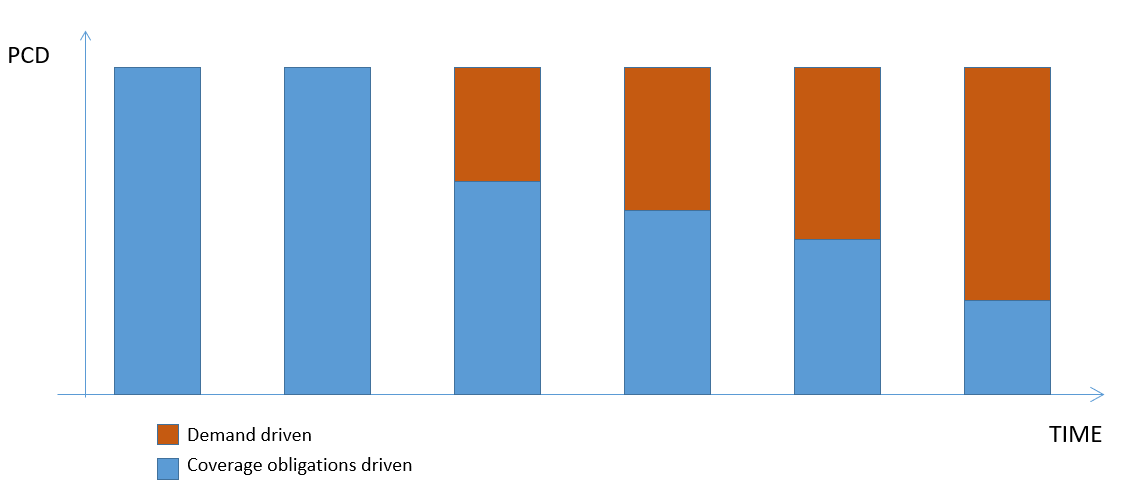
\includegraphics[width=4.6in,height=2.0in]{./media/image104.png}
		%\caption{Impact of the coverage obligations in the end-user speed. Source: Author}
%
	%\end{Center}
%\end{figure}
%
%
%%%%%%%%%%%%%%%%%%%%% Figure/Image No: 7 Ends here %%%%%%%%%%%%%%%%%%%%
%
%\par
%
%Third. Having information at a PCD level is not detailed enough for the propagation model. Obtaining information about the percentage of the urban, suburban and rural area of each PCD would allow MINERVA to have more precise simulations. The same issue applies to the percentage of penetration of mobile services. It is currently set at 80$\%$ , but this percentage shall depend on the geotype since they use mobile services for different use cases.\par
%
%Fourth. This work only takes into account the traditional traffic generated by end users but does not consider the other possible use cases of the 5G networks: Massive machine-type communications and Ultra-reliable and low latency communications. Each use case conditions 5G networks in a different way and all of them should be considered in the model. Thus, MINERVA should consider issues such as that some traffic types will demand low rate connections and that IoT communications could exceed the maximum simultaneous connections allowed to a base station. MINERVA should include models of these types of traffic and consider them in the decision module.\par
%
%
%%Fifth. The model could also consider a more complex analysis of the consumer experience and Volker Stocker and Jason Whalley suggest in this paper.\par
%
%%\href{https://www.sciencedirect.com/science/article/pii/S0308596116302142}{https://www.sciencedirect.com/science/article/pii/S0308596116302142}\par